\documentclass[11pt]{article}
\usepackage[T1]{fontenc}
\usepackage[utf8]{inputenc}
\usepackage{lmodern}
\usepackage[margin=1.05in]{geometry}
\usepackage{amsmath,amssymb,amsthm,mathtools}
\usepackage{microtype}
\usepackage{enumitem}
\usepackage{tikz-cd}
\usepackage{xcolor}
\usepackage[colorlinks=true,linkcolor=blue!45!black,citecolor=blue!45!black,urlcolor=blue!45!black]{hyperref}
\usepackage{bookmark}
\usepackage{xurl}
\usepackage{doi}
\setlength{\emergencystretch}{2em}
\numberwithin{equation}{section}
\newtheorem{theorem}{Theorem}[section]
\newtheorem{proposition}[theorem]{Proposition}
\newtheorem{lemma}[theorem]{Lemma}
\newtheorem{corollary}[theorem]{Corollary}
\theoremstyle{definition}
\newtheorem{definition}[theorem]{Definition}
\newtheorem{remark}[theorem]{Remark}
\newcommand{\C}{\mathbb C}
\newcommand{\Q}{\mathbb Q}
\newcommand{\R}{\mathbb R}
\newcommand{\Z}{\mathbb Z}
\newcommand{\OO}{\mathcal O}
\newcommand{\PP}{\mathbb P}
\newcommand{\cJ}{\mathcal J}
\newcommand{\cG}{\mathcal G}
\newcommand{\cM}{\mathcal M}
\newcommand{\ddc}{dd^c}
\DeclareMathOperator{\ord}{ord}
\DeclareMathOperator{\divisor}{div}
\DeclareMathOperator{\rk}{rk}
\DeclareMathOperator{\td}{td}
\DeclareMathOperator{\Supp}{Supp}
\DeclareMathOperator{\Pic}{Pic}
\DeclareMathOperator{\Isom}{Isom}
\DeclareMathOperator{\codim}{codim}
\DeclareMathOperator{\ch}{ch}

\title{Invariant anticanonical indices and conversion of twisted differentials}
\author{OpenAI}
\date{September 26, 2026}
\hypersetup{pdftitle={Invariant anticanonical indices and conversion of twisted differentials},pdfauthor={OpenAI}}
\begin{document}
\maketitle
\begin{abstract}
For a holomorphic action of a compact torus on a compact complex manifold,
we prove that the invariant Euler characteristic of naturally linearized
anticanonical powers is polynomial on a divisible progression, with its
actual value at exponent zero. Independently, on a smooth projective
variety with smoothly semipositive anticanonical bundle, we remove a fixed
pseudoeffective error from an unbounded sequence of effective twists.
These results convert invariant cohomology into twisted differential
forms and prove anticanonical nonvanishing on smooth projective varieties
with smoothly semipositive anticanonical bundle, by descending the forms
before conversion.
\end{abstract}
\section{Introduction}
\label{sec:introduction}

Two questions about anticanonical bundles motivate this paper. First,
when a torus acts on a compact complex manifold, can the invariant Euler
characteristic at the trivial power force invariant cohomology at large
anticanonical powers? Second, on a smooth projective variety, can a fixed
pseudoeffective error be removed from an unbounded sequence of effective
anticanonical twists? We answer the first question without a positivity
assumption and the second under smooth metric semipositivity. They meet
in an application to differential forms: invariant cohomology supplies
forms that descend through monodromy, and conversion is applied only
after that descent.

\subsection{The invariant index and its value at zero}

Let \(T\) be a compact real torus acting smoothly by holomorphic
automorphisms on a compact complex manifold \(F\). Its differential
acts on the anticanonical line \(L_F=-K_F=\det T_F\). We call this
the \emph{natural linearization}. The corresponding action on a section
is \((t\cdot s)(x)=t_{L_F}s(t^{-1}x)\); tensor powers carry the induced
action. For each integer \(m\ge0\), define
\[
I_T(m)=\sum_{q\ge0}(-1)^q\dim H^q(F,L_F^m)^T.
\]
Thus \(I_T(m)\) is the multiplicity of the trivial representation in the
Dolbeault index of \(L_F^m\).

\begin{theorem}[Invariant anticanonical index]\label{thm:index}
Let a compact real torus \(T\) act holomorphically on a compact complex
manifold \(F\), and give \(-K_F\) its natural linearization.
There are an integer \(a>0\) and a polynomial \(P\in\Q[t]\) such that
\[
I_T(m)=P(m)\quad\text{for every positive multiple \(m\) of \(a\)},
\qquad P(0)=I_T(0).
\]
\end{theorem}

The theorem has no projectivity, K\"ahlerness, or positivity premise.
Its endpoint is essential: when \(I_T(0)\ne0\), the polynomial cannot
vanish at all large divisible exponents. Some fixed cohomological degree
therefore contains invariant classes at unbounded exponents. Eventual
polynomiality alone would give no information about whether that
polynomial is zero.

The natural linearization is equally essential. On a point, twisting the
trivial line by a nonzero torus character gives invariant dimension zero
at every positive power and dimension one at power zero. For the natural
anticanonical action, by contrast, the fiber character at a fixed
component is the sum of the normal tangent characters. This identity
controls the endpoint.

Our calculation uses the holomorphic Lefschetz framework of
Atiyah--Bott \cite{AtiyahBott1966} and its compact-group, fixed-component
form due to Atiyah--Segal and Atiyah--Singer
\cite{AtiyahSegal1968,AtiyahSinger1968}. Polarizing its denominators
expresses the invariant multiplicity as polynomially weighted lattice
counts on rational polytopes with specified coordinate faces removed.
Weighted Ehrhart theory supplies polynomiality on divisible exponents
\cite[preprint \S2.4 and \S3.1]{BaldoniBerlineDeLoeraKoeppeVergne2012}.
To determine the value at zero, we prove the count directly, retaining
all small divisible exponents, and then show that the anticanonical
character gives a deformation retraction onto the removed faces.
The cancellation is a difference of Euler characteristics of compact
polyhedra. Stanley's treatment of deleted boundary already identifies
this constant term and singles out boundary visible from an exterior
point
\cite[Proposition~8.2 and the discussion and proof of Proposition~8.3]{Stanley1974Reciprocity}.
Here the anticanonical character produces such an exterior point in the
affine counting space. We give a direct weighted argument and an explicit
retraction, including degenerate polytopes.

When \(F\) is K\"ahler and \(L_F\) has a smooth semipositive metric,
hard Lefschetz with semipositive coefficients
\cite[Theorem~0.1]{DPS2001} gives
\[
H^0(F,\Omega_F^{n-q}\otimes L_F^{m+1})
\longrightarrow H^q(F,L_F^m),\qquad n=\dim F,
\]
surjectively. An invariant K\"ahler form makes this map equivariant;
compact averaging then preserves surjectivity on invariant subspaces.
The coefficient is \(L_F^{m+1}\) because the cohomological target is
\(K_F\otimes L_F^{m+1}=L_F^m\). Thus Theorem~\ref{thm:index} supplies
invariant twisted differential forms when \(I_T(0)\ne0\).
The use of hard Lefschetz and a nonzero Euler characteristic to obtain
infinitely many twisted forms already appears for canonical powers in
\cite[Theorem~2.7.3]{DPS2001}; here the invariant anticanonical index
requires a separate argument to retain its value at exponent zero.

\subsection{Removing a fixed error}

We use additive notation for line bundles and Cartier divisors. A divisor
is \emph{pseudoeffective} if its numerical class lies in the closure of
the effective cone. Smooth semipositivity means the existence of a smooth
Hermitian metric with nonnegative Chern curvature; it implies nefness.
The next theorem is an ordinary section theorem, with no group action.

\begin{theorem}[Pseudoeffective-error conversion]\label{thm:conversion}
Let \(S\) be a smooth connected projective complex variety, and suppose
that \(L=-K_S\) has a smooth Hermitian metric with semipositive Chern
curvature. Let \(D\) be a pseudoeffective Cartier divisor. If
\[
H^0(S,\OO_S(m_jL-D))\ne0
\]
for a strictly increasing sequence of positive integers \(m_j\), then
\(H^0(S,\OO_S(kL))\ne0\) for some integer \(k>0\).
\end{theorem}

The fixed error need not be effective. No rational-connectedness or
Euler-characteristic assumption on \(S\) is used. The argument begins
with a rational map whose base has maximal dimension among maps
\(S\dashrightarrow Y\) for which a multiple of \(L\) dominates an
ample base divisor in pseudoeffective order. Maximality forces ratios
of the relevant sections to be base functions. Their horizontal zero
orders consequently vary affinely with the exponent.

After birational modifications, a normalization along base divisors
produces a line bundle \(B\) on a smooth base \(Y\) and a nonzero map
\[
\sigma:f^*B\longrightarrow\ell\pi^*L,\qquad \ell>0,
\]
where \(V\) is smooth, \(\pi:V\to S\) is birational, and
\(f:V\to Y\) is a morphism. This map will be used to transfer the
sections constructed on the base to positive multiples of \(L\) on
\(S\). The same maximality gives
rank-one adjoint direct images, whose integral metrics yield a
semipositive metric on \(B\) by Berndtsson's positivity theorem
\cite{Berndtsson2009}. The normalization of \(\sigma\) makes the
resulting weights locally bounded, including near singular fibers.

These bounds allow Fujino's Koll\'ar--Nadel theorem \cite{Fujino2018}
to give vanishing at every nonnegative base twist. A single Euler
polynomial therefore equals the corresponding section dimension even
at zero, where the exceptional canonical section makes it positive.
Some positive exponent gives a section, which \(\sigma\) transfers
back to \(S\). As in the invariant-index argument, control at zero
is what rules out the zero polynomial; the two constructions of that
control are independent.

This criterion applies to differential forms through a determinant
construction. The generic-span method of Lazi\'c--Peternell
\cite[Lemma~4.1]{LP2018}, adapted in
Lazi\'c--Matsumura--Peternell--Tsakanikas--Xie
\cite[Lemma~5.1]{LMPTX2023}, extracts one fixed determinant line
from infinitely many twisted forms. We give the argument for an
unbounded positive sequence, including the numerically trivial case
excluded by the hypotheses of those two cited lemmas. The cotangent
subsheaf theorem \cite[Theorem~4.1]{LMPTX2023}, with Ou's generic
nefness result \cite[Theorem~1.4]{Ou2023} as an antecedent, makes the
negative of that line pseudoeffective. Theorem~\ref{thm:conversion}
then removes the error.

\subsection{Application through monodromy}

For a smooth connected projective \(X\), anticanonical nonvanishing asks
for a section of \(-mK_X\) for some \(m>0\). The positive-multiple
question under smooth semipositivity is associated with Yau's
anticanonical-section problem \cite[Problem~75]{Yau1994}.
The prescribed-Ricci theorem \cite{Yau1978} and the structure theorems
of Demailly--Peternell--Schneider and Campana--Demailly--Peternell
\cite{DPS1996,CDP2015} identify a compact rationally connected factor
of the universal cover. Residual monodromy can still act on it through
a compact torus, so a section on that factor alone need not descend.
M\"uller's equivariant theorem produces invariant plurisections under
semiampleness \cite[Theorem~C]{Muller2025}.
His Theorem~A proves nonvanishing for projective klt pairs with nef
anti-log-canonical divisor when its restriction to the general fiber of
the maximal rationally connected fibration is semiample; Corollary~B
proves nonvanishing for projective klt threefold pairs with nef
anti-log-canonical divisor. Our smooth application assumes metric
semipositivity and imposes no fiber-semiampleness condition.

We apply the invariant index on the compact factor \(F\) and ordinary
conversion on a finite cover \(S\) of \(X\); descending forms is the
step that connects those two spaces.

The companion \emph{Anticanonical nonvanishing from smooth
semipositivity} \cite{CompanionH} proves a finite-cover description with the
residual torus and invariant canonical frames retained, as well as the
finite \'etale norm of a section. We use only these
geometric inputs. We prove locally that invariant twisted forms on the
compact factor descend injectively to the finite cover. Theorem~\ref{thm:index}
and hard Lefschetz provide those forms, and
Theorem~\ref{thm:conversion} is applied after descent. Taking the norm
then proves that \(-mK_X\) has a nonzero section for some \(m>0\).

Passing to a positive multiple is necessary. On an Enriques surface
\(E\), \(K_E\) has order two and \(H^0(E,-K_E)=0\)
\cite{Dolgachev2016}. Consequently \(E\times\PP^1\) has a smoothly
semipositive, non-torsion anticanonical bundle without a first-power
section. In dimension two, the classification of
Chen--Filip--Sun--Tosatti--Zhang
\cite[Theorem~1.3]{CFSTZ2026} gives complementary geometric
context.\footnote{Their introduction credits ChatGPT~5.6~Sol with
suggesting a preliminary version of Lemma~5.2, which the authors
reformulated and developed into its geometric statement and proof.}

Section~\ref{sec:index} proves the index theorem and derives invariant
twisted forms. Section~\ref{sec:conversion} proves conversion by
constructing the normalized relative section and bounded base metric.
Section~\ref{sec:differentials} gives the determinant argument.
Section~\ref{sec:descent} proves form descent and the global application.
The two principal theorems are independent of one another; their
combination takes place only in that last application.

\section{The invariant index, including exponent zero}
\label{sec:index}

The proof of Theorem~\ref{thm:index} rests on two facts about weighted
lattice counts, which we establish before applying localization.
Here is the counting problem that explains their role. For a fixed
component, polarization of the fixed-point formula produces integral vectors
\(\alpha_1,\ldots,\alpha_s,w\in\Z^r\), where \(r=\dim T\), and a subset
\(I\subset\{1,\ldots,s\}\). Its counting equation is
\[
\sum_{i=1}^s\alpha_i b_i=-mw,
\qquad b_i>0\ (i\in I),\quad b_i\ge0\ (i\notin I).
\]
The vectors \(\alpha_i\) are positive under one linear functional;
\(w\) is the natural anticanonical character; and \(I\) records
the denominators whose expansions
start at a positive exponent. Section~\ref{subsec:localization} derives
these data from the normal tangent action. For now this equation explains
the two counting tasks.

First, the closed count, in which every inequality is weak, is polynomial
at every divisible exponent; its polynomial value at zero is the weight
at zero. Second, imposing the strict inequalities removes coordinate
faces. The anticanonical character gives a retraction onto their union,
so its Euler characteristic cancels the constant of the closed count.
Only the constant terms from contributions with no deleted faces survive.
At actual exponent
\(m=0\), positivity of the \(\alpha_i\) forces \(b=0\), allowed
exactly in that same case. Matching these two endpoint calculations
completes the index proof.

Polynomially weighted Ehrhart sums and fundamental parallelepipeds are
classical; see
\cite[preprint \S2.4 and \S3.1]{BaldoniBerlineDeLoeraKoeppeVergne2012}.
We give the count directly to retain the low divisible powers and the
value at zero, before proving the special deleted-face assertion.

\begin{lemma}[A weighted lattice count at zero]\label{lem:ehrhart}
Let \(D\subset\R^s\) be a nonempty closed rational polytope, and
let \(W(x,m)\) be a polynomial in \(x\) and \(m\).
For sufficiently divisible positive integers \(m\),
\[
\sum_{x\in mD\cap\Z^s}W(x,m)
\]
is polynomial in \(m\), and its polynomial value at zero is \(W(0,0)\).
The same assertion holds with coefficients in any finite-dimensional
vector space.
\end{lemma}

\begin{proof}
Choose a positive integer \(a\) clearing all vertex denominators.
Writing \(m=an\), replace \(D\) by the lattice polytope \(aD\) and
the weight by \(W(x,an)\). Its value at \((0,0)\) is unchanged.
We may therefore prove the assertion for a lattice polytope and again
call the dilation variable \(m\). Triangulate into closed lattice
simplices, using lattice vertices. It suffices first to treat a
\(d\)-dimensional simplex with vertices \(v_0,\ldots,v_d\).

The vectors \((v_i,1)\) are linearly independent. Use the lattice
\(\Z^{s+1}\cap\operatorname{span}_{\R}\{(v_i,1):0\le i\le d\}\)
in their real linear span. Every lattice point in their nonnegative
cone has a unique expression
\[
p+\sum_{i=0}^d l_i(v_i,1),\qquad l_i\in\Z_{\ge0},
\]
where \(p\) is a lattice point of the half-open fundamental
parallelepiped for these generators. This permits a lower-dimensional
simplex, a nonunimodular simplex, and a simplex not containing the
origin. The height \(h\) of \(p\) is an integer with
\(0\le h\le d\), and height \(m\) imposes
\(\sum l_i=m-h\).
For fixed \(p\), substitute this expression into \(W\) and expand the
resulting polynomial in the basis
\(\prod_i\binom{l_i}{u_i}\), with coefficients polynomial in \(m\).
The identity
\begin{equation}\label{eq:binomial}
\sum_{\substack{l_i\ge0\\\sum l_i=m-h}}
\prod_{i=0}^d\binom{l_i}{u_i}
=
\binom{m-h+d}{d+\sum_i u_i}
\end{equation}
follows by multiplying the generating functions
\(z^{u_i}/(1-z)^{u_i+1}\).
For \(m\ge h\) it is the desired counting identity.
For \(0\le m<h\), the upper entry on the right is an integer between
zero and \(d-1\), so the binomial polynomial also vanishes.
Thus the polynomial formula is valid for every \(m\ge0\).

At \(m=0\), every term with \(h>0\) vanishes. The only parallelepiped
point of height zero is the origin. For it, only \(u_i=0\) for all \(i\)
contributes in \eqref{eq:binomial}, giving \(W(0,0)\).
This proves the assertion for a simplex of any dimension.

Apply inclusion--exclusion to the closed simplices in the triangulation.
Each nonempty intersection is a lattice face and has the same constant
term \(W(0,0)\). The alternating sum of these constant terms is
\(\chi(D)W(0,0)=W(0,0)\), because a nonempty convex polytope is
contractible. The vector-valued assertion follows coefficientwise.
\end{proof}

\subsection{The deleted boundary}

Polarizing a fixed-point denominator may exclude some coordinate faces.
The next lemma proves the cancellation needed for those exclusions.
Its geometry is simple: a point outside the nonnegative orthant lies
in the affine space containing the polytope, and rays from that point
first enter the polytope through the faces being removed.

\begin{lemma}[Deleted faces]\label{lem:faces}
Let \(\alpha_1,\ldots,\alpha_s\) be vectors admitting a linear
functional positive on each, and let \(I\subset\{1,\ldots,s\}\).
Put \(u_i=-1\) for \(i\in I\), \(u_i=1\) otherwise, and set
\[
D=\left\{x_i\ge0:\ \sum_i\alpha_ix_i=\sum_i\alpha_iu_i\right\}.
\]
If \(D\ne\varnothing\) and \(I\ne\varnothing\), the union
\[
A=\bigcup_{i\in I}\bigl(D\cap\{x_i=0\}\bigr)
\]
is a deformation retract of \(D\). In particular \(\chi(A)=1\).
\end{lemma}

\begin{proof}
The positivity of the functional makes \(D\) compact.
For \(x\in D\), put
\[
t(x)=\max_{i\in I}\frac1{x_i+1},\qquad
r(x)=u+t(x)(x-u).
\]
Then \(0<t(x)\le1\), and \(r(x)\) lies in the same affine equation
space as \(x\) and \(u\).
For \(i\in I\), its \(i\)-th coordinate is
\(-1+t(x)(x_i+1)\ge0\), with equality for at least one index.
For \(i\notin I\), it is \(1-t(x)+t(x)x_i\ge0\).
Hence \(r(x)\in A\).
If \(x\in A\), then \(t(x)=1\), so \(r(x)=x\).
The continuous straight homotopy from \(x\) to \(r(x)\) stays in the
convex set \(D\) and fixes \(A\). This proves the assertion.
\end{proof}

Figure~\ref{fig:deleted-face} illustrates this retraction when all three
vectors \(\alpha_i\) are \(1\) and \(I=\{1\}\). The proof above
also applies when \(D\) has smaller dimension or consists of one point.

\begin{figure}[htbp]
\centering
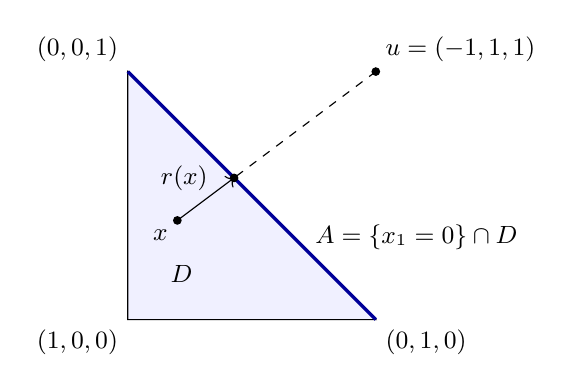
\begin{tikzpicture}[scale=1.05, every node/.style={font=\small}]
\coordinate (U) at (3,3);
\coordinate (Eone) at (0,0);
\coordinate (Etwo) at (3,0);
\coordinate (Ethree) at (0,3);
\coordinate (X) at (.6,1.2);
\coordinate (R) at (1.285714,1.714286);
\fill[blue!6] (Eone)--(Etwo)--(Ethree)--cycle;
\draw (Eone)--(Etwo)--(Ethree)--cycle;
\draw[very thick,blue!60!black] (Etwo)--(Ethree);
\draw[dashed] (U)--(R);
\draw[->] (X)--(R);
\fill (U) circle (1.5pt) node[above right] {\(u=(-1,1,1)\)};
\fill (X) circle (1.5pt) node[below left] {\(x\)};
\fill (R) circle (1.5pt) node[left=6pt] {\(r(x)\)};
\node[below left] at (Eone) {\((1,0,0)\)};
\node[below right] at (Etwo) {\((0,1,0)\)};
\node[above left] at (Ethree) {\((0,0,1)\)};
\node at (.65,.55) {\(D\)};
\node[right] at (2.15,1.0) {\(A=\{x_1=0\}\cap D\)};
\end{tikzpicture}
\caption{The affine plane \(x_1+x_2+x_3=1\), drawn using
\((x_2,x_3)\) as coordinates. The triangle is \(D\), and its thick
edge is the deleted union \(A\). The point \(r(x)\) is the first
point of \(D\) on the ray from \(u\) through \(x\); the homotopy
moves \(x\) along the indicated segment to that edge.}
\label{fig:deleted-face}
\end{figure}

\begin{remark}[The visible-face alternative]\label{rem:visible-faces}
Stanley discusses the visible-boundary case in
\cite[discussion preceding and proof of Proposition~8.3]{Stanley1974Reciprocity}.
Here it also gives a short geometric proof covering degenerate polytopes.
With \(D\ne\varnothing\) and \(I\ne\varnothing\), the preceding
coordinate calculation identifies \(A\) as exactly the first entry
points of rays from \(u\) into \(D\). Indeed, for \(a\in A\),
a coordinate with \(a_i=0\), \(i\in I\), stays negative on the
segment from \(u\) preceding \(a\).
By strict separation, choose a linear functional \(f\) and \(c>0\) with
\(f(x-u)>c\) on \(D\), and project centrally onto
\(H=\{z:f(z-u)=c\}\):
\[
\pi(x)=u+\frac{c(x-u)}{f(x-u)}.
\]
There is one first entry point on each ray meeting \(D\), so
\(\pi|_A\) is a continuous bijection onto \(\pi(D)\), hence a
homeomorphism by compactness. The image is convex: it is the section
by \(H\) of the convex cone with vertex \(u\) generated by \(D\).
Thus \(A\) is homeomorphic to a nonempty compact convex set and
\(\chi(A)=1\), also for lower-dimensional and singleton polytopes.
Both proofs concern \(\chi(D)-\chi(A)\); one must not replace
that difference by the ordinary Euler characteristic of the nonclosed
set \(D\setminus A\).
\end{remark}

\subsection{Localization and the anticanonical character}
\label{subsec:localization}

We now identify the lattice domains in the fixed-point formula. The two
lemmas above will determine their constant terms component by component.

\begin{proof}[Proof of Theorem~\ref{thm:index}]
Write \(\Lambda=\operatorname{Hom}(T,S^1)\) for the character lattice
and \(t^\lambda\) for the value at \(t\in T\) of a character
\(\lambda\in\Lambda\). The invariant index is the coefficient of
\(t^0\) in the alternating character.

The Dolbeault complex is an equivariant elliptic complex on any compact
complex manifold; a K\"ahler metric is not needed for its index.
For elements generating dense cyclic subgroups of \(T\), the fixed
locus is \(F^T\). If \(F^T\) is empty, the fixed-point theorem makes
the entire alternating character zero on these elements. Such elements
are dense in \(T\), and the character of a finite-dimensional virtual
representation is continuous, hence identically zero. In this case
\(I_T(m)=0\) for all \(m\), including zero, and we take \(P=0\).
Otherwise apply the equivariant Dolbeault fixed-point formula on the
dense set of these elements. Clearing its finitely many denominators
gives an identity of rational characters.
Its compact-group form, including fixed components, follows from
\cite[Theorem~2.12 and \S3]{AtiyahSegal1968} and
\cite[Theorems~3.9 and 4.3]{AtiyahSinger1968}.
For a component \(Z\) of \(F^T\), write \(\nu_i\ne0\) for the normal
tangent characters, repeated with their ranks, and \(x_i\) for the
corresponding formal Chern roots. The natural anticanonical fiber
weight is
\[
w=\sum_i\nu_i.
\]
Writing \(L=K_F^{-1}\), the contribution to the alternating character
is
\begin{equation}\label{eq:localization}
\int_Z \td(Z)\,e^{m c_1(L|_Z)}\,t^{mw}
\prod_i\frac1{1-t^{-\nu_i}e^{-x_i}}.
\end{equation}
The action on sections uses the inverse action on arguments, accounting
for the conormal characters in the denominator.
Choose an integral one-parameter direction pairing nontrivially with
every normal character at every fixed component.
For a component \(Z\), let \(I\) be the indices with positive pairing.
Put \(\alpha_i=\nu_i\) on \(I\), and \(\alpha_i=-\nu_i\) otherwise.
All \(\alpha_i\) pair positively with the chosen direction.
The pairings are positive integers, hence at least one.
Expand the denominators toward exponents with positive pairing:
\[
\frac1{1-t^{-\nu_i}e^{-x_i}}
=
\begin{cases}
-\displaystyle\sum_{b_i>0}t^{b_i\alpha_i}e^{b_ix_i},
&i\in I,\\[6pt]
\displaystyle\sum_{b_i\ge0}t^{b_i\alpha_i}e^{-b_ix_i},
&i\notin I.
\end{cases}
\]
These expansions respect the identity of rational characters in a
completion in which there are only finitely many terms below each
pairing bound. In particular, each trivial-character coefficient is
a finite sum.

The coefficient of the trivial character in \eqref{eq:localization}
is therefore a polynomially weighted lattice count satisfying
\[
\sum_i\alpha_i b_i=-mw,\qquad
b_i>0\ (i\in I),\quad b_i\ge0\ (i\notin I).
\]
Before integration, the polynomial weight in the truncated root space is
\begin{equation}\label{eq:lattice-weight}
W(b,m)=(-1)^{|I|}\left[
\td(Z)\exp\!\left(m c_1(L|_Z)
 +\sum_{i\in I}b_i x_i-\sum_{i\notin I}b_i x_i\right)
\right]_{\le\dim Z}.
\end{equation}
The bracket retains complex cohomological degrees at most \(\dim Z\),
so only finitely many terms contribute and \(W\) is polynomial in
\(b,m\). The sign is part of this weight.
All root expressions are interpreted by the splitting principle in
truncated cohomological degrees. Operations are first performed
coefficientwise with formal roots. Individual root monomials or
individual face terms need not define cohomology classes. Permuting
roots within an equal-character normal bundle, together with the
corresponding lattice coordinates, preserves the entire lattice domain
and its total weighted sum. Thus the complete sum is symmetric at
every positive divisible exponent. Its polynomial continuation is
symmetric coefficient by coefficient, by uniqueness of a polynomial
on an infinite progression. Only after taking this complete sum do we
interpret the symmetric polynomials as characteristic classes and
integrate on \(Z\).

For positive \(m\), the domain is the dilation by \(m\) of the rational
compact polytope
\begin{equation}\label{eq:D}
D=\left\{b_i\ge0:\ \sum_i\alpha_i b_i=-w\right\},
\end{equation}
with the union \(A\) of its faces \(b_i=0\), \(i\in I\), removed.

If \(I=\varnothing\), then \(-w=\sum_i\alpha_i\), so \(D\ne\varnothing\).
Lemma~\ref{lem:ehrhart} gives the polynomial continuation, whose
constant term is the weight at \((b,m)=(0,0)\).
If \(I\ne\varnothing\) and \(D\) is empty, the contribution is zero.
Otherwise the vector with coordinates \(-1\) on \(I\) and \(1\)
elsewhere belongs to the affine equation space in \eqref{eq:D},
since the linearization is anticanonical.
Lemma~\ref{lem:faces} gives \(\chi(A)=\chi(D)=1\).
By inclusion--exclusion and Lemma~\ref{lem:ehrhart}, the polynomial
constant term of the count on \(D\setminus A\) is
\[
\bigl(\chi(D)-\chi(A)\bigr)W(0,0)=0.
\]

These constants are exactly the actual trivial-character contributions
at \(m=0\). Indeed, positivity of the pairing forces every \(b_i=0\)
when \(\sum\alpha_i b_i=0\); this is permitted precisely when
\(I=\varnothing\). Summing over fixed components and taking a common
divisibility integer proves both polynomiality and \(P(0)=I_T(0)\).
An empty normal list gives the one-point lattice domain in \(\R^0\),
with no deleted faces; its contribution is the ordinary index integral
on that fixed component. This also handles a trivial torus. The empty
fixed set was handled before localization.
Finally, the polynomial has rational coefficients because its values at
all positive points of an integral progression are integers.
\end{proof}

\subsection{Invariant twisted forms}

The index theorem is independent of positivity. For its geometric
application we now assume K\"ahlerness and introduce the analytic map
that turns cohomology into holomorphic forms.

\begin{theorem}[Hard Lefschetz with semipositive coefficients]
\label{thm:lef}
Let \(F\) be compact Kähler of dimension \(n\), with Kähler form
\(\omega\), and let \(A\) have a smooth semipositive Hermitian metric.
For every \(0\le q\le n\), wedge multiplication by \(\omega^q\) induces a
surjection
\[
H^0(F,\Omega_F^{n-q}\otimes A)
\longrightarrow H^q(F,K_F\otimes A).
\]
\end{theorem}

This is the smooth-metric case of
\cite[Theorem~0.1]{DPS2001}; its multiplier ideal is trivial.
The smooth-coefficient Lefschetz theorem of Mourougane
\cite[Theorem~2.6]{Mourougane1999} and the earlier nef-coefficient
cohomology work of Takegoshi \cite[Theorem~1]{Takegoshi1997} are
antecedents of this statement. We use the formulation in \cite{DPS2001}.
If a compact group preserves the data, the map is equivariant. Averaging
over the group then preserves surjectivity on invariant subspaces.

\begin{corollary}\label{cor:invariantforms}
Let \(F\) be compact Kähler with smoothly semipositive
\(L_F=-K_F\), and let a compact torus \(T\) act holomorphically,
with the natural linearization on \(L_F\). If
\[
\sum_q(-1)^q\dim H^q(F,\OO_F)^T\ne0,
\]
then for some fixed \(p\ge0\) and arbitrarily large positive integers
\(m\),
\[
H^0(F,\Omega_F^p\otimes L_F^{m+1})^T\ne0.
\]
\end{corollary}

\begin{proof}
By Theorem~\ref{thm:index}, \(I_T(m)\ne0\) for all but finitely many
positive integers in a divisible progression. Some fixed \(q\)
therefore has \(H^q(F,L_F^m)^T\ne0\) for unbounded \(m\).
Average a Kähler form over \(T\), and apply
Theorem~\ref{thm:lef} with \(A=L_F^{m+1}\). Its target is
\[
H^q(F,K_F\otimes L_F^{m+1})=H^q(F,L_F^m).
\]
The wedge map is equivariant, and compact averaging gives an invariant
preimage of each invariant target class. Take \(p=\dim F-q\).
Indeed the map is \(u\mapsto[\omega^q\wedge u]\); it depends on the
averaged K\"ahler form and the natural linearization, not on the
coefficient metric used to establish surjectivity. Averaging a chosen
preimage over Haar probability measure therefore leaves its invariant
target unchanged.
\end{proof}

\section{Removing a pseudoeffective error}
\label{sec:conversion}

We prove Theorem~\ref{thm:conversion}. Throughout this section
\(L=-K_S\) carries a fixed smooth semipositive metric, and we choose
effective integral divisors
\begin{equation}\label{eq:effective-sequence}
N_j\sim m_jL-D,\qquad m_1<m_2<\cdots.
\end{equation}
We use additive notation for line bundles. A divisor is pseudoeffective
when its numerical class lies in the closed effective cone; on a smooth projective variety
it is equivalent to admitting a singular Hermitian metric with
semipositive curvature current \cite{DPS2001}. Such classes pull back
under dominant maps between smooth projective varieties and push forward
under birational morphisms. 

The proof builds a resolution \(\pi:V\to S\), a morphism
\(f:V\to Y\), and a line bundle \(B\) on the base, together with
a nonzero map \(f^*B\to\ell\pi^*L\). The map will be used to transfer the
sections constructed on the base to positive multiples of \(L\) on
\(S\). Its normalization will also supply
the bounds needed to construct those base sections.

\subsection{The base and the relative section}

\paragraph{A maximal base.}
Call a dominant rational map \(S\dashrightarrow Y\) \emph{dominated
by \(L\)} if, after resolving it to a morphism \(f:V\to Y\),
\begin{equation}\label{eq:domination}
c\pi^*L-f^*H\quad\text{is pseudoeffective}
\end{equation}
for some positive integer \(c\) and ample Cartier divisor \(H\) on
the integral projective variety \(Y\). The constant map is allowed:
the trivial line on a point is ample, and \(L\) is pseudoeffective.
There is therefore a dominated map of largest possible base dimension.

We may choose its base smooth and its function field relatively
algebraically closed in \(\C(S)\). Indeed, normalize the original
base in its relative algebraic closure in \(\C(S)\), a finite
extension, and then resolve the base and the rational map. The pullback
of the original ample divisor to the new smooth base is big. A large
multiple of this pullback dominates an ample divisor in pseudoeffective
order, which preserves \eqref{eq:domination}. The same argument permits
further birational modifications of the base and higher smooth source
models.

This choice has a useful maximality property. If \(A\) is a line
bundle on \(S\) and \(c'L-A\) is pseudoeffective for some
\(c'>0\), then the ratio of any two nonzero sections of \(A\)
lies in \(\C(Y)\). To prove this, suppose their ratio is nonconstant
and resolve the corresponding pencil. Its moving line is the pullback
of \(\OO_{\PP^1}(1)\), and its fixed divisor is effective, so the
pencil is dominated by \(L\). The joint map of this pencil and
\(S\dashrightarrow Y\) is dominated as well: add their two
inequalities on a common resolution and restrict the ample product
line to the joint image. Normalizing and resolving that image preserves
domination. By maximality its dimension is \(\dim Y\), so the
pencil's function is algebraic over \(\C(Y)\). Relative algebraic
closedness places it in \(\C(Y)\), as asserted. A constant ratio
already has this property. When necessary, increasing \(c'\) to an
integer preserves pseudoeffectivity because \(L\) is pseudoeffective.

Apply this property to the effective divisors in
\begin{equation}\label{eq:interpolation}
(m_j-m_2)N_1+(m_2-m_1)N_j
\sim(m_j-m_1)N_2,\qquad j>2.
\end{equation}
Their common class is \((m_j-m_1)(m_2L-D)\), which is bounded
above by \((m_j-m_1)m_2L\) in pseudoeffective order. The equivalence
function in \eqref{eq:interpolation} thus belongs to \(\C(Y)\).
On any normal model resolving the map to \(Y\), a prime is called
\emph{horizontal} if it dominates \(Y\), and \emph{vertical} otherwise.
A base function has order zero at a horizontal prime. If \(a_j\) is
the coefficient of the pullback of \(N_j\) at such a prime, then
\eqref{eq:interpolation} gives
\[
a_j=a_1+\frac{m_j-m_1}{m_2-m_1}(a_2-a_1).
\]
Since \(a_j\ge0\) along an unbounded sequence, \(a_2\ge a_1\).
Consequently the pullback of \(N_2-N_1\) has effective horizontal part.

If \(Y\) is a point, apply this calculation on \(S\) itself: every
prime is horizontal, and \(N_2-N_1\) is effective. Its class is
\((m_2-m_1)L\), proving the theorem in this case. Henceforth
\(\dim Y>0\). The remaining task is to remove the negative vertical
coefficients by subtracting a divisor from the base.

\paragraph{Normalization along base divisors.}
For that subtraction to see every vertical coefficient, we need each
vertical prime to dominate a base divisor. We construct a normal
intermediate model with this property:
\[
\begin{tikzcd}[column sep=large]
V\arrow[r,"\rho"]\arrow[dr,bend right=15,"f"']&
U\arrow[r,"b"]\arrow[d,"h"]&S\\
&Y&
\end{tikzcd}
\qquad \pi=b\rho,\quad f=h\rho.
\]
Here \(b\) and \(\rho\) are birational, \(V\) and \(Y\) are
smooth projective, and every prime divisor of \(U\) that fails to
dominate \(Y\) dominates a prime divisor of \(Y\).

For this construction, begin with a smooth resolution \(V_0\to Y_0\)
of the maximal map. On a dense open of \(Y_0\), its fibers form a
flat family of subschemes of \(V_0\) with a fixed Hilbert polynomial.
Resolve the induced rational map from \(Y_0\) to the projective
Hilbert scheme, obtaining a smooth projective birational base \(Y\)
\cite[Theorem~3.2, p.~260; p.~265]{Grothendieck1961Hilbert}.
Pull back the universal family. Every fiber of this family has
dimension \(r=\dim S-\dim Y\). The reduced closure \(W\) of the
original flat family is integral and maps birationally to \(V_0\).
Its fibers are closed subschemes of the pulled-back Hilbert fibers,
so have dimension at most \(r\). The normalization \(U\to W\)
is finite, and hence has the same fiber-dimension bound over \(Y\).
A prime divisor \(Q\subset U\) mapping into a subset of codimension
at least two would satisfy
\[
\dim Q\le \dim Y-2+r=\dim S-2,
\]
which is impossible. Resolve \(U\) to obtain \(V\). The dimension
bound is needed on \(U\); the smooth space \(V\) will be used for
metrics and vanishing. The preceding maximality argument preserves
\eqref{eq:domination} throughout these modifications.

On this model, let \(s_0\) be the rational section of
\((m_2-m_1)b^*L\) whose divisor is \(b^*(N_2-N_1)\). Its horizontal
part is effective by the preceding calculation. The base divisor to
be subtracted is now determined one prime at a time.

For each prime divisor \(P\subset Y\), subtract the smallest
normalized vertical order:
\begin{equation}\label{eq:minima}
b_P=\min_{Q\mapsto P}
\frac{\ord_Q(s_0)}{\ord_Q(h^*P)}.
\end{equation}
The minimum runs over the finitely many components of \(h^*P\)
dominating \(P\). This set is nonempty and its denominators are
positive. Only finitely many \(b_P\) are nonzero, because
\(\divisor(s_0)\) has finite support. Every vertical prime of \(U\)
occurs in one of these minima. Together with horizontal effectivity,
this proves
\[
\divisor(s_0)-h^*\Bigl(\sum_P b_PP\Bigr)\ge0.
\]
Choose a positive integer \(a\) clearing all denominators and set
\[
\ell=a(m_2-m_1),\qquad B=a\sum_Pb_PP.
\]
Smoothness of \(Y\) makes \(B\) Cartier. On the normal variety
\(U\), the resulting rational section of \(\ell b^*L-h^*B\)
has nonnegative order at every prime, so is regular. Pulling it back
to \(V\) gives
\begin{equation}\label{eq:sigma}
\sigma:\OO_V(f^*B)\longrightarrow\OO_V(\ell\pi^*L).
\end{equation}
For every base prime \(P\), some component of \(f^*P\) dominating
\(P\) has order zero in \(\sigma\): take the strict transform of
a prime attaining \eqref{eq:minima}. Its strict transform defines the
same divisorial valuation, since \(U\) is normal and hence regular
at its generic point. The new exceptional divisors on \(V\) acquire
no poles because the pulled-back section is regular. This is the
normalization we will use near singular fibers; equidimensionality of
\(V\) is unnecessary.

\paragraph{Rank one of the adjoint direct images.}
We now have the map that will transfer sections from the base. To
construct a semipositive metric on its source line \(B\), we will
use adjoint integral metrics. Their direct images must first be shown
to have rank one. The anticanonical identity enters at this point. Put
\begin{equation}\label{eq:discrepancy}
E=K_V-\pi^*K_S=K_V+\pi^*L.
\end{equation}
The divisor \(E\) is effective and \(\pi\)-exceptional; denote its
canonical section by \(e\). For every integer \(k\ge0\), we claim
that
\begin{equation}\label{eq:rank-one}
\cG_k=f_*\OO_V(E+k\ell\pi^*L)
\quad\text{has generic rank one.}
\end{equation}
The section \(e\sigma^k\), after trivializing \(B\) over the
generic point, shows that the rank is at least one, also when \(k=0\).
If it were larger, Serre's global generation theorem would give, for
some positive \(t\), two sections of
\(E+k\ell\pi^*L+tf^*H\) independent over \(\C(Y)\). Their ratio
would lie outside that field.

Push their zero divisors forward to \(S\). They become two effective
divisors in one Cartier class
\[
A\sim k\ell L+t\pi_*f^*H,
\]
with the same rational-function ratio. Indeed, choose a Cartier divisor
representing the upstairs line and express both sections as rational
functions; birational pushforward preserves their principal divisors,
and \(\pi_*E=0\). Smoothness makes the common downstairs divisor
Cartier. Pushing forward \eqref{eq:domination} gives
\[
(k\ell+tc)L-A\quad\text{pseudoeffective}.
\]
The maximality property then places the ratio in \(\C(Y)\), a
contradiction. The coefficient \(k\ell+tc\) is positive even at
\(k=0\), proving \eqref{eq:rank-one} in its full stated range.

\subsection{The bounded base metric}

We have constructed \(B\) and \(\sigma\); the next task is a
semipositive metric on \(B\) with locally bounded weights. For a local
frame \(\beta\), our weight convention is \(-\log|\beta|^2\),
so semipositive curvature means that the weights are plurisubharmonic.
We obtain them as limits of adjoint integral metrics. We use
Berndtsson's direct-image theorem in the following
form \cite[Theorem~1.2]{Berndtsson2009}: for a proper holomorphic
submersion with K\"ahler total space and a smoothly semipositive line
bundle \(A\), the natural \(L^2\) metric on
\(f_*(K_{V/Y}+A)\) has semipositive curvature wherever the adjoint
sections form a vector bundle. The coefficient metric may be
semipositive; strict positivity along the fibers is not required.

Let \(h_L\) denote the pulled-back smooth metric on \(\pi^*L\).
Choose a dense Zariski open \(Y^\circ\) on which \(f\) is smooth
and \(e\) and \(\sigma\) are not identically zero on any fiber.
The fibers there are connected: relative algebraic closedness of
\(\C(Y)\) in \(\C(S)\) makes the finite part of the Stein
factorization trivial. For a local frame \(\beta\) of \(B\), set
\(\sigma_\beta=\sigma(f^*\beta)\) and
\begin{equation}\label{eq:max-weight}
\varphi_\beta(y)=-\log\max_{V_y}
|\sigma_\beta|_{h_L^\ell}^{\,2},\qquad y\in Y^\circ.
\end{equation}
The fiberwise maximum is positive and continuous on this open set.

To see that \(\varphi_\beta\) is plurisubharmonic, take a local
frame \(\tau\) of \(K_Y\). Equation~\eqref{eq:discrepancy} gives
\begin{equation}\label{eq:adjoint}
K_{V/Y}+(1+k\ell)\pi^*L
=E+k\ell\pi^*L-f^*K_Y.
\end{equation}
Thus \(e\sigma_\beta^k/f^*\tau\) is an adjoint section. By
\eqref{eq:rank-one} and generic base change, it spans the adjoint
direct image on a dense open subset of \(Y^\circ\). For every
integer \(k\ge1\), Berndtsson's theorem makes
\begin{equation}\label{eq:moment-weights}
\varphi_{\beta,k}(y)
=-\frac1k\log\int_{V_y}
|\sigma_\beta|_{h_L^\ell}^{\,2k}
\left|e/f^*\tau\right|_{h_L}^{\,2}
\end{equation}
plurisubharmonic on that dense open. The integral is smooth and
strictly positive throughout \(Y^\circ\); its curvature inequality
therefore holds on all of \(Y^\circ\) by continuity.

The final factor in the integral is the smooth nonnegative measure
obtained from a \(\pi^*L\)-valued relative canonical form. It has
positive mass and full support on each fiber, because a nonzero
holomorphic section on a connected smooth fiber cannot vanish on an
open subset. Denote this measure by \(\mu_y\), its mass by
\(M(y)>0\), and put
\[
q_\beta=|\sigma_\beta|_{h_L^\ell}^{\,2},\qquad
A_k(y)=\left(\frac1{M(y)}\int_{V_y}q_\beta^k\,d\mu_y\right)^{1/k}.
\]
H\"older's inequality for the probability measure \(M(y)^{-1}\mu_y\)
shows that \(A_k(y)\) increases with \(k\). Full support gives
\(A_k(y)\to\max_{V_y}q_\beta\). The moments and their limit are
continuous, so Dini's theorem makes this convergence uniform on every
compact subset of a coordinate open in \(Y^\circ\). The limit is
positive there. Since
\[
\varphi_{\beta,k}=-\log A_k-\frac1k\log M,
\]
the weights in \eqref{eq:moment-weights} converge locally uniformly to
\(\varphi_\beta\). Their limit is plurisubharmonic.

It remains to establish local bounds near the omitted fibers.
Properness of \(f\) and smoothness of the upstairs metric bound
\(q_\beta\) above over every relatively compact base neighborhood.
Equation~\eqref{eq:max-weight} therefore gives a local lower bound
for \(\varphi_\beta\), even as one approaches the boundary.

For the upper bound, let \(P\) be a divisorial component of
\(Y\setminus Y^\circ\). The normalization of \(\sigma\) supplies
a component \(Q\) above \(P\) on which \(\sigma\) is generically
nonzero. Choose a general point of \(Q\) where \(P,Q\) are smooth,
\(Q\to P\) is submersive, no other component of \(f^*P\) passes
through the point, and \(\sigma\ne0\). In suitable local coordinates, a
transverse coordinate to \(P\) pulls back to a unit times \(z_1^r\),
with \(r>0\), while the other base coordinates pull back to independent
coordinates along \(Q\). Taking a local root absorbs the unit.
This local form shows that a small source neighborhood maps onto a
base neighborhood. On a still smaller source neighborhood,
\(q_\beta\) has a positive lower bound. Every sufficiently nearby
fiber meets this neighborhood, so its maximum has the same lower
bound. This gives an upper bound for \(\varphi_\beta\) near a
general point of \(P\).

The removable-singularity theorem for plurisubharmonic functions now
extends \(\varphi_\beta\) across dense open subsets of all boundary
divisors. These opens can be taken Zariski open: nonvanishing and the
required differential ranks hold on algebraic opens of \(Q\), whose
dominant constructible images contain dense Zariski opens of \(P\).
The set still omitted is therefore contained in a closed analytic set
\(A\subset Y\) of codimension at least two.

We recall why no upper-bound obstruction remains at \(A\). Near a
point of \(A\), choose a small affine complex disk centered there whose
boundary misses \(A\), and a compact neighborhood of that boundary disjoint
from \(A\). The plurisubharmonic function has a common upper bound
on this neighborhood. For every nearby \(y\notin A\), choose a disk
of the same radius centered at \(y\), with direction sufficiently
close to the original one that its boundary stays in this fixed
neighborhood. Its direction can also be chosen so that the whole
disk misses \(A\):
the radial image of \(A\), viewed from \(y\), in the space of complex line directions
has real dimension at most \(2\dim Y-4\), smaller than the direction
space dimension \(2\dim Y-2\). The submean inequality gives
a common upper bound at all such \(y\). Removable singularities
therefore extend the function across \(A\) as well. The upper-limit
extension preserves the lower bound already supplied by properness.

We have obtained locally bounded plurisubharmonic weights on all of
\(Y\). Under \(\beta'=g\beta\), formula~\eqref{eq:max-weight}
gives
\[
\varphi_{\beta'}=\varphi_\beta-\log|g|^2.
\]
The same relation holds after extension, so the weights define a
semipositive singular Hermitian metric \(h_B\) on \(B\), with
locally bounded weights.

\subsection{Vanishing at every nonnegative exponent}

The bounded metric on \(B\) is now available. To produce sections,
we combine it with a metric on \(\pi^*L\) that is positive in base
directions and has no multiplier-ideal loss. Recall that \(\cJ(h)\)
consists locally of holomorphic functions \(g\) for which
\(|g|^2e^{-\varphi_h}\) is integrable.

The domination \eqref{eq:domination} gives a singular metric on
\(\pi^*L\) whose curvature is positive in base directions. More
precisely, combine a semipositive singular metric on
\(c\pi^*L-f^*H\) with a positive smooth metric on \(H\), and take
the \(c\)-th root. The resulting metric \(h_1\) satisfies
\[
\Theta_{h_1}(\pi^*L)\ge c^{-1}f^*\omega_H.
\]
Mix its local weights with those of the smooth semipositive metric
\(h_L\): for some \(0<\delta<1\), put
\(h=h_L^{1-\delta}h_1^\delta\). The local exponential-integrability consequence of Skoda's theorem
\cite[Proposition~7.1, p.~389]{Skoda1972} supplies, near each point,
a sufficiently small positive exponent for which the negative
exponential of the singular weight is integrable. We use its
arbitrary-plurisubharmonic-weight formulation in
\cite[Definition~0.1 and 1.4(8)]{DemaillyKollar2001}:
for a nontrivial psh weight \(\varphi\), the local integrability
threshold of \(e^{-2\gamma\varphi}\) is positive. This formulation
also includes complex dimension one. In our squared-norm convention,
take \(\gamma=\delta/2\). A finite coordinate
cover of the compact space \(V\) gives one common \(\delta>0\).
The smooth part changes integrability by bounded factors. Hence
\begin{equation}\label{eq:small-metric}
\Theta_h(\pi^*L)\ge\epsilon f^*\omega_H,
\qquad \cJ(h)=\OO_V,
\qquad \epsilon=\delta/c>0.
\end{equation}

For each integer \(k\ge0\), tensor this metric with \(f^*h_B^k\).
Its curvature is still at least \(\epsilon f^*\omega_H\), and its
multiplier ideal is still trivial: for every fixed \(k\), the added
weight is locally bounded. Thus the same choice of \(h\) works at
all the required exponents.

We use Fujino's Koll\'ar--Nadel vanishing theorem in the following
form \cite[Theorem~1.3]{Fujino2018}. If \(f:V\to Y\) is a
surjective morphism from a compact K\"ahler manifold to a projective
variety and a line bundle \(A\) has a singular metric \(h_A\) with
\(\Theta_{h_A}(A)\ge\epsilon f^*\omega_H\), then
\[
H^i\bigl(Y,R^qf_*(\OO_V(K_V+A)\otimes\cJ(h_A))\bigr)=0
\qquad (i>0,\ q\ge0).
\]
Fujino derives this form from the injectivity and multiplier-ideal
Bertini theorems of Fujino--Matsumura
\cite[Theorems~1.1--1.3]{Fujino2018}. The metric need not have analytic
singularities. Apply the theorem to
\(A=\pi^*L+kf^*B\), with the metric just constructed, and take \(q=0\). Since
\(K_V+\pi^*L=E\), the projection formula gives
\begin{equation}\label{eq:all-vanishing}
H^i\bigl(Y,\cG\otimes\OO_Y(kB)\bigr)=0
\qquad(i>0,\ k\ge0),
\qquad \cG=f_*\OO_V(E).
\end{equation}

Riemann--Roch on the smooth projective base makes
\[
Q(k)=\chi\bigl(Y,\cG\otimes\OO_Y(kB)\bigr)
=\int_Y\ch(\cG)e^{k c_1(B)}\td(Y)
\]
a polynomial in \(k\), whether or not \(B\) is ample. By
\eqref{eq:all-vanishing}, this polynomial equals
\(h^0(Y,\cG\otimes\OO_Y(kB))\) at every nonnegative integer.
At zero the canonical section \(e\) gives a nonzero section, so
\(Q(0)>0\). This is why vanishing at \(k=0\) is indispensable:
without it, the existence of \(e\) would not determine the Euler
characteristic. The polynomial is nonzero, and hence cannot vanish
at every positive integer. For some \(k>0\) there is a nonzero
section of \(E+kf^*B\) on \(V\).

Multiply this section by \(\sigma^k\) from \eqref{eq:sigma}. The
result is a nonzero section of \(E+k\ell\pi^*L\). Finally,
\(\pi_*\OO_V(E)=\OO_S\): a rational function with possible poles
only on the effective exceptional divisor \(E\) is regular away
from its codimension-two image, and extends across that image by
normality of \(S\). The projection formula therefore sends our
section to a nonzero section of \(k\ell L\), completing the proof
of Theorem~\ref{thm:conversion}.

The two appearances of \(L=-K_S\) explain the strength and the scope
of the criterion. The identity \(K_V+\pi^*L=E\) supplies the
adjoint section used in the integral metric and turns adjoint
vanishing into the fixed sheaf \(f_*\OO_V(E)\) at exponent zero.
These steps connect the positive base metric to an Euler polynomial
with a known nonzero value.

\section{From twisted differentials to effective divisors}
\label{sec:differentials}
Theorem~\ref{thm:conversion} accepts any fixed pseudoeffective error.
We now construct one from differential forms, so that the invariant
forms obtained in Section~\ref{sec:index} can be used after descent.
The construction has two steps: take a fixed determinant line of a generic
span, then control the sign of that line by generic nefness.

\begin{theorem}[Cotangent subsheaves]\label{thm:subsheaf}
Let \(S\) be smooth projective with \(-K_S\) nef.
If a line bundle \(M\) is a saturated subsheaf of
\((\Omega_S^1)^{\otimes b}\), where \(b>0\), then \(-M\) is
pseudoeffective.
\end{theorem}

This is the smooth, zero-boundary, rank-one case of
\cite[Theorem~4.1]{LMPTX2023}; Ou's generic-nefness theorem
\cite[Theorem~1.4]{Ou2023} is an antecedent of the cotangent result.

\begin{lemma}[Determinants of twisted differentials]\label{lem:determinant}
Let \(S\) be smooth connected projective with \(-K_S=L\) nef.
Suppose that, for a fixed \(p>0\),
\[
H^0(S,\Omega_S^p\otimes\OO_S(mL))\ne0
\]
for arbitrarily large positive integers \(m\).
Then there is a pseudoeffective Cartier divisor \(D\) and a strictly
increasing sequence \(d_j>0\) with effective integral divisors
\[
N_j\sim d_jL-D.
\]
\end{lemma}

The generic-span construction below adapts
\cite[Lemma~4.1]{LP2018} and \cite[Lemma~5.1]{LMPTX2023}. We give the
proof for the present unbounded positive sequence, including the
numerically trivial case excluded by the numerical-nontriviality
premises of those two cited lemmas, and include the saturation argument needed
for the negative first-Chern-class conclusion of
\cite[Theorem~4.1]{LMPTX2023}.

\begin{proof}
Choose one nonzero section at each of an unbounded set of exponents.
Over \(\C(S)\), trivialize \(L\) rationally and let \(W\) be the
span of the chosen vectors. Take a basis \(u_1,\ldots,u_r\) of \(W\)
from among them. For infinitely many unbounded exponents, the corresponding
vector has nonzero coefficient along one fixed \(u_a\). Wedging that
section with the other \(r-1\) basis sections gives a nonzero section
of
\[
\bigwedge\nolimits^r\Omega_S^p\otimes\OO_S(d_jL),
\]
where, if the fixed basis sections have exponents \(a_1,\ldots,a_r\),
the new exponent is \(d_j=m_j+\sum_{i\ne a}a_i\).
The sum is fixed, so the \(d_j\) are unbounded and may be taken strictly increasing.
Every such wedge spans the same line \(\bigwedge^r W\).

Let \(M\) be its saturation in \(\bigwedge^r\Omega_S^p\).
A saturated rank-one subsheaf of a vector bundle on a smooth variety
is reflexive: its double dual maps into that vector bundle by extension
across codimension two, and any enlargement would give torsion in the
quotient. Hence \(M\) is a line bundle. Each wedge factors through
\(M(d_jL)\), since its image in the torsion-free quotient is generically
zero.

In characteristic zero, exterior powers are direct summands of tensor
powers. Thus \(\bigwedge^r\Omega_S^p\) is a direct summand of
\((\Omega_S^1)^{\otimes rp}\), and \(M\) remains saturated in that
tensor power: the additional summand is a vector bundle, so the enlarged
quotient is still torsion-free. Theorem~\ref{thm:subsheaf} makes \(D=-M\)
pseudoeffective. The zero divisors of the induced nonzero sections of
\(M(d_jL)\) are the required \(N_j\).
\end{proof}

\begin{corollary}[Conversion of twisted differentials]\label{cor:conversion}
Let \(S\) be smooth connected projective with smoothly semipositive
\(L=-K_S\). If, for one fixed \(p\ge0\),
\[
H^0(S,\Omega_S^p\otimes\OO_S(mL))\ne0
\]
for arbitrarily large positive integers \(m\), then some positive
multiple of \(L\) has a nonzero section.
\end{corollary}

\begin{proof}
For \(p=0\) this is immediate. For \(p>0\), apply
Lemma~\ref{lem:determinant} and Theorem~\ref{thm:conversion}.
\end{proof}

\section{Descent before conversion}
\label{sec:descent}

We now combine the two principal theorems. The geometric input describes
a finite cover while retaining its residual torus action. Invariant forms
on a compact factor then descend to that cover, where the ordinary
conversion theorem applies.

We use the following finite-cover structure statement from
\cite[Theorem~(Finite cover with compact torus monodromy)]{CompanionH}. If \(X\) is smooth
connected projective and \(-K_X\) is smoothly semipositive, there is
a connected finite \'etale projective cover
\(\nu:S\to X\) whose universal cover is
\[
\widetilde S=\C^b\times C\times F.
\]
Here \(C\) and \(F\) are compact simply connected projective factors;
\(C\) is Ricci-flat, and \(F\) has smoothly semipositive anticanonical
bundle and no positive-degree holomorphic forms. The deck group acts by
translations on \(\C^b\), trivially on \(C\), and through a compact
real torus \(T\) of holomorphic isometries on \(F\). The first two
factors have nowhere-zero holomorphic canonical forms invariant under
the deck group. Empty products are points and have unit canonical frame.

The proof of this statement in the companion starts from Yau's
prescribed-Ricci theorem and the Ricci-semipositive structure theory
\cite{Yau1978,DPS1996,CDP2015}. Its finite-cover construction preserves
monodromy and the invariant frames. It also proves the vanishing of
holomorphic forms by the Bochner argument on irreducible
non-Ricci-flat factors, independently of the rational-connectedness
conclusion of the refined structure theorem. K\"ahler Hodge symmetry
therefore gives
\begin{equation}\label{eq:factor-euler}
H^q(F,\OO_F)=0\quad(q>0),\qquad H^0(F,\OO_F)=\C,
\qquad I_T(0)=1.
\end{equation}
This deduction includes a point factor.

\begin{proposition}[Descent of invariant twisted forms]\label{prop:descent}
Let \(\nu:S\to X\), \(F\), and \(T\) be the finite-cover data just
specified. After choosing invariant canonical frames on \(\C^b\) and
\(C\), there is, for every \(r\ge0\) and \(0\le p\le\dim F\), an
injective linear map
\[
H^0(F,\Omega_F^p\otimes(-K_F)^r)^T
\longrightarrow H^0(S,\Omega_S^p\otimes(-K_S)^r).
\]
For some fixed \(p\), the target is nonzero at unbounded positive
integers \(r\).
\end{proposition}

\begin{proof}
Let \(\eta\) be the product of the chosen canonical frames on
\(\C^b\) and \(C\). For an invariant form \(u\) in the displayed
source, pull back its differential part along the projection to \(F\)
and use \(\eta^{-r}\) for the other anticanonical factors. This gives
\[
\eta^{-r}\otimes\operatorname{pr}_F^*u
\in H^0\bigl(\widetilde S,
\Omega_{\widetilde S}^p\otimes K_{\widetilde S}^{-r}\bigr).
\]
Translations preserve the Euclidean frame, the action on \(C\) is
trivial, and the action on \(F\) lies in \(T\), with its natural induced
action on both tensor factors of \(u\). The tensor is therefore
deck-invariant and descends holomorphically to \(S\). Pullback along
the projection is injective on differential forms, tensoring with
\(\eta^{-r}\) is invertible, and local covering charts preserve
nonvanishing. Hence the descent map is injective. Its holomorphic
sections are algebraic because \(S\) is projective.

By \eqref{eq:factor-euler} and Corollary~\ref{cor:invariantforms}, there
are a fixed \(p\) and invariant sections in
\(H^0(F,\Omega_F^p\otimes(-K_F)^{m+1})\) for unbounded positive
\(m\). Apply the constructed map with \(r=m+1\). If \(F\) is a
point, its constant section gives the same assertion with \(p=0\).
\end{proof}

\begin{corollary}[Smooth anticanonical nonvanishing]\label{cor:global}
Let \(X\) be a smooth connected projective complex variety. If
\(-K_X\) has a smooth Hermitian metric with semipositive Chern
curvature, then \(H^0(X,-mK_X)\ne0\) for some integer \(m>0\).
\end{corollary}

\begin{proof}
Choose the finite cover above. Proposition~\ref{prop:descent} gives
nonzero anticanonically twisted differential forms on \(S\) in one
fixed degree and at unbounded positive exponents. The anticanonical
metric on \(S\) is the smooth semipositive pullback metric. Apply
Corollary~\ref{cor:conversion} on \(S\) to obtain a nonzero section of
\(-kK_S\), \(k>0\).

The finite \'etale norm of a section
\cite[Lemma~(Finite \'etale norm)]{CompanionH} sends a nonzero section of
\(\nu^*A\) to a nonzero section of \(A^{\otimes d}\), where
\(d=\deg\nu\); a Galois hypothesis is unnecessary. With
\(A=-kK_X\), the identity \(K_S=\nu^*K_X\) therefore gives a section
of \(-dkK_X\). For zero-dimensional connected \(X\), the canonical
line is trivial and the assertion is immediate.
\end{proof}

The ordering of the argument matters. The torus-invariant objects are
the forms on \(F\); they descend before any section-conversion theorem
is applied. Consequently no equivariant strengthening of
Theorem~\ref{thm:conversion} is required, and the finite cover is never
treated as a global product.

\begingroup
\small
\bibliographystyle{plain}
\bibliography{references}
\endgroup
\end{document}
